\chapter{Courants induits}
\section{Expérience}
Une bobine est reliée à un voltmètre, un aimant est placé dans la bobine. Lorsque l'aimant est brusquement retiré de la bobine, le voltmètre indique qu'un courant temporaire s'est formé dans le circuit. Le courant ainsi créé est appelé \motcle{courant induit} et, avec les piles qui utilisent les réactions d'oxydo-réduction, il s'agit des méthodes les plus largement utilisées pour produire de l'électricité.

Dans ce chapitre, nous étudierons les courants induits ainsi que les concepts théoriques nécessaires à leur étude.

\section{Paramètres affectant le courant induit}
Il existe plusieurs façons de modifier l'importance du courant induit :
\begin{itemize}[label=\textbullet]
    \item utiliser un aimant différent
    \item retirer l'aimant plus rapidement
    \item faire varier l'orientation de la bobine par rapport au champ magnétique
\end{itemize}

Il est également possible de modifier le sens du courant induit si on retourne l'aimant ou s'il est approché de la bobine au lieu de l'éloigner.
\begin{figure}[ht]
    \centering
    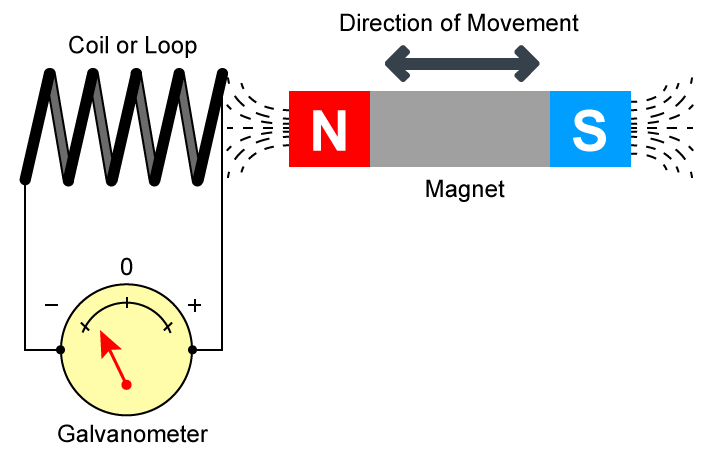
\includegraphics[width=0.5\linewidth]{induction_I.png}
    \caption{La variation de flux crée un courant induit.}
    \label{induction_I}
\end{figure}

\section{Le flux magnétique}
Si des aimants différents permettent d'induire des courants différents, c'est parce qu'ils ne génèrent pas autour d'eux des champs magnétiques de même intensité. Il est donc nécessaire de connaître la quantité de magnétisme qui traverse une spire de la bobine.
La valeur totale du champ magnétique traversant une surface, par exemple celle formée par une spire, est appelée \motcle{flux magnétique}.

\begin{encadre}
    \motcle{flux magnétique} : \(\Phi [Weber]\)
\end{encadre}

Seule la composante du champ magnétique perpendiculaire à la surface est utile au flux, dès lors, lorsque le champ est uniforme et la surface plane, le flux se calcule en faisant le produit scalaire entre B et S :

\begin{encadre_equation*}{Flux magnétique à travers une surface régulière}
    \begin{equation}
        \begin{split}
            \Phi & = \vec{B} \cdot \vec{S} \\
            \Phi & = ||\vec{B}|| \cdot ||\vec{S}|| \cdot cos \theta
        \end{split}
    \end{equation} où :
    \begin{itemize}[label=\textbullet]
        \item \( \Phi \)  est le flux magnétique en [Wb] ;
        \item \( \vec{B} \) est le vecteur champ magnétique en [T];
        \item \( \theta\) est l'angle entre \( \vec{B} \) et \( \vec{S} \)
        \item \( \vec{S} \) est le vecteur surface en \([m^2]\),
              \begin{itemize}
                  \item son intensité correspond à la valeur de la surface,
                  \item sa direction est toujours perpendiculaire à celle-ci.
              \end{itemize}
    \end{itemize}
\end{encadre_equation*}

\begin{figure}[ht]
    \centering
    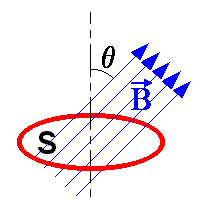
\includegraphics[width=0.2\linewidth]{flux_magnetique.png}
    \caption{Le flux magnétique est la valeur totale du champ B traversant perpendiculairement la surface S.}
    \label{flux_magnetique}
\end{figure}

\newpage

\section{Flux magnétique sur une surface non plane et dans un champ non-uniforme (hors programme)}
La situation présentée à la page précédente est un cas simple, le champ est uniforme et la surface est plane. Comment peut-on calculer le flux lorsque la situation est plus complexe ?

\begin{figure}[ht]
    \centering
    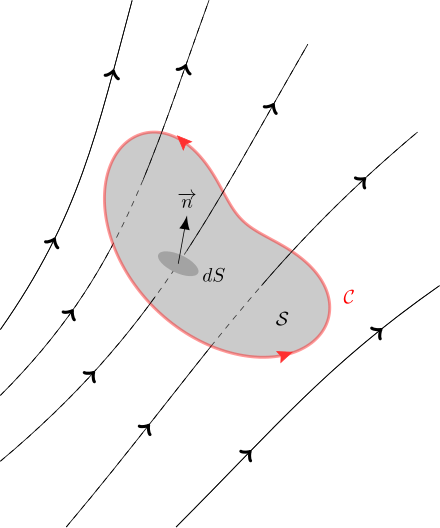
\includegraphics[width=0.5\linewidth]{flux_magnetique_II.png}
    \caption{Un champ magnétique non uniforme traversant une surface quelconque.}
    \label{flux_magnetique_II}
\end{figure}

Dans ce cas, il va falloir découper la surface \(S\) en une infinité de morceaux infiniment petits et calculer la somme de tous les éléments de flux pour l'ensemble des éléments de surface. Cette technique, est rendue possible par le \motcle{calcul intégral} que tu aborderas cette année en math. Dans ce cas :
\(\Phi =  \int \vec{B} \cdot \vec{dS}\), où \(\vec{dS}\) est un élément de surface infiniment petit.

\newpage

\section{Exercices}
\begin{exercise}
    Quelle est la valeur du flux magnétique à l'intérieur d'un carré de \(10[cm]\) de côté traversé par un champ magnétique uniforme de \(0,2[T]\) si les lignes de champ forment un angle de \(30^{\circ}\) par rapport à la normale au cadre ?
\end{exercise}

\begin{exercise}
    Quel doit être le rayon d'une boucle circulaire de fil conducteur se trouvant dans un champ de \(0,07[T]\) pour qu'un flux de \(4[Wb]\) traverse cette boucle? Le plan de la boucle est perpendiculaire aux lignes de champ.
\end{exercise}

\newpage

\section{Loi de Lenz : sens du courant induit}
Lorsque le flux magnétique varie à l'intérieur d'une spire, un courant induit se forme dans celle-ci. Or, tu sais que le passage d'un courant dans une spire produit lui-même un champ magnétique.
Quel est alors le lien entre le champ magnétique extérieur et le champ magnétique induit ? Vont-ils s'additionner ou se soustraire ?
La loi de Lenz répond à cette question :

\begin{encadre}
    \motcle{Loi de Lenz} : les effets de la force électromotrice\footnotemark{} induite sont tels qu'ils s'opposent à la variation de flux qui les a produits.
\end{encadre}
\footnotetext{Le terme \enquote{force électromotrice} prête à confusion, il ne s'agit pas d'une force, mais de l'énergie électrique qu'un dispositif comme une pile ou une bobine peut communiquer à une charge de un Coulomb. Si on néglige la résistance interne du dispositif alors la force électromotrice correspond à la \textbf{différence de potentiel} aux bornes de celui-ci.}

On utilise la loi de Lenz pour déterminer le sens du courant induit.

\subsection{Analyses de cas}
\begin{itemize}
    \item Le pôle Nord d'un aimant est approché d'une spire (Figure~\ref{loi_lenz}, schéma de gauche), le flux au sein de la spire causé par le champ magnétique extérieur va augmenter et un champ magnétique induit s'opposant au champ extérieur va apparaître. La règle du tire-bouchon permet de retrouver le sens du courant dans la spire.
    \item Si pôle Nord de l'aimant est ensuite éloigné de la spire  (Figure~\ref{loi_lenz}, schéma de droite), le flux diminue et le champ induit sera dirigé dans le même sens que le champ extérieur puisque le champ induit tend à maintenir le flux. La règle du tire-bouchon nous montre que dans ce cas le courant sera dans le sens inverse à la première situation.
\end{itemize}

\newpage

\begin{figure}[ht]
    \centering
    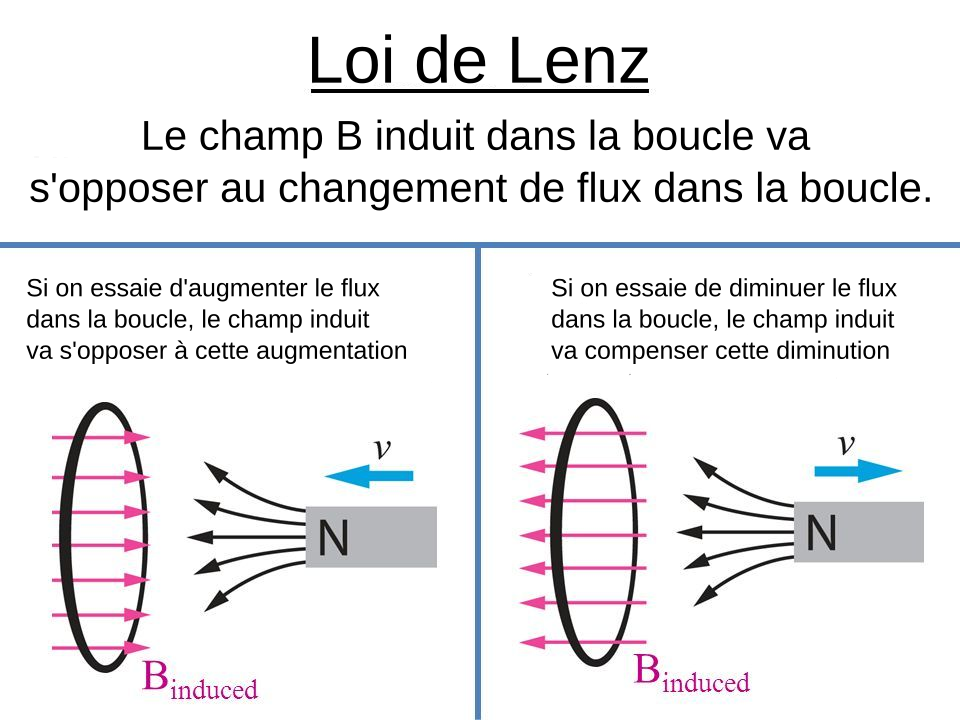
\includegraphics[width=\linewidth]{loi_lenz.png}
    \caption{La loi de Lenz}
    \label{loi_lenz}
\end{figure}

\newpage

\subsection{Exercice}

\begin{exercise}
    Le pôle Sud d'un aimant est éloigné d'une spire, quel sera le sens du courant induit dans celle-ci ? Fait un schéma.
\end{exercise}

\begin{figure}[ht]
    \centering
    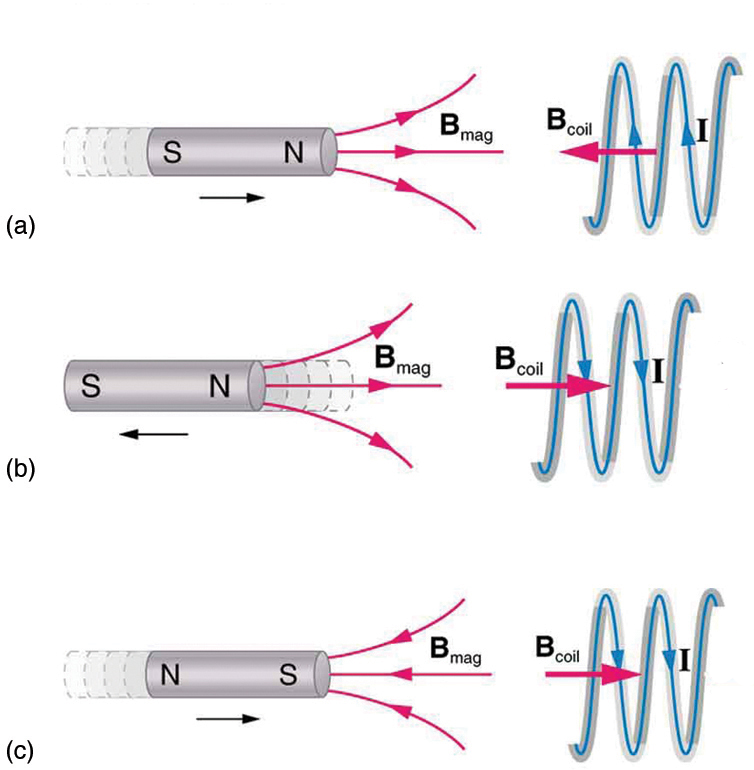
\includegraphics[width=\linewidth]{loi_lenz_II.png}
    \caption{La loi de Lenz}
    \label{loi_lenz_2}
\end{figure}

\newpage

\section{Loi de Faraday : valeur de la différence de potentiel induite}
La loi de Faraday permet de connaître la différence de potentiel \footnote{Il s'agit en fait de la force électromotrice, mais l'usage de ce terme prêtant à confusion, une simplification est faite en assimilant la f.e.m à la différence de potentiel.} induite dans une spire ou une bobine, dans le cas d'une variation constante.

Considérons un cadre en U fermé par un barreau pouvant glisser dessus. L'ensemble est plongé dans un champ magnétique uniforme entrant. Le barreau est déplacé vers la droite d'une distance \(\Delta x\).\begin{figure}[h!]
    \centering
    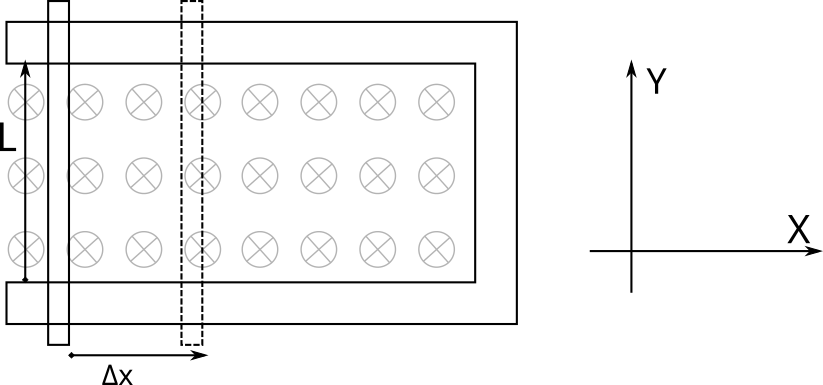
\includegraphics[width=.6\linewidth]{loi_faraday.png}
    \label{loi_faraday}
\end{figure}

\newpage

Dans cette situation, nous savons que le flux dans la spire diminue, un courant induit se forme donc de manière à maintenir ce flux. Le champ induit sera, lui aussi, entrant et le courant induit sera de sens horloger.
La variation de flux est égale à :
\begin{equation}\label{faraday_1}
    \Delta \Phi = B \cdot \Delta S
\end{equation}

La variation de surface est causée par une variation de la largeur, \(\Delta x\), la hauteur \enquote{L} est constante. Donc :

\begin{equation}\label{faraday_2}
    \Delta \Phi = - B \cdot L \cdot \Delta x
\end{equation}

Le signe \enquote{-} apparaît, car la surface diminue,  \(\Delta S\) est négatif.

La variation de flux engendre un courant induit dans le barreau, mais ce dernier est situé dans un champ magnétique. Une force électromagnétique (force de Laplace) s'exerce donc sur lui dans le sens inverse de l'axe de X. Elle vaut :

\begin{equation}\label{faraday_3}
    F_{Laplace} = B \cdot I \cdot L
\end{equation}

À cause de la force de Laplace, il faut pousser sur le barreau pour pouvoir le déplacer. La force avec laquelle il faut pousser le barreau, \(F_{mot}\), est égale à la force de Laplace :
\begin{equation}\label{faraday_4}
    F_{mot}= F_{Laplace}
\end{equation}

Pour pouvoir déplacer le barreau, il a fallu exercer une force dessus, \(F_{mot}\), mais lorsqu'une force permet un déplacement, elle effectue un travail.
\begin{equation}\label{faraday_5}
    W_{mot} = \vec{F_{mot}} \cdot \vec{\Delta x}
\end{equation}

Puisque \(F_{mot} = F_{Laplace}\), les relations \ref{faraday_3} et \ref{faraday_5} peuvent être combinées :
\begin{equation}\label{faraday_6}
    W_{mot} = B \cdot I \cdot L \cdot \Delta x
\end{equation}

Étant donné que \(\Delta \Phi = - B \cdot L \cdot \Delta x \) (relation \ref{faraday_2}),  alors l'équation précédente (relation \ref{faraday_6}) peut s'écrire :
\begin{equation}\label{faraday_7}
    W_{mot} = - \Delta \Phi \cdot I
\end{equation}

Il faut maintenant se demander ce que devient l'énergie, \(W_{mot}\), dépensée lors du déplacement du barreau. L'énergie ne peut ni apparaître, ni disparaitre. Celle du travail moteur est en fait convertie en énergie électrique. Donc :
\begin{equation}\label{faraday_8}
    W_{mot}=W_{elec}
\end{equation}

L'énergie électrique dépensée ou reçue dans un circuit est donnée par :
\begin{equation}\label{faraday_9}
    W_{elec}=U \cdot I \cdot \Delta t
\end{equation}

Les équations \ref{faraday_7} et \ref{faraday_9} peuvent être combinées, ce qui donne
\begin{equation}
    - \Delta \Phi \cdot I = U \cdot I \cdot \Delta t
\end{equation}

Par conséquent :
\begin{equation}
    U = - \frac{\Delta \Phi}{\Delta t}
\end{equation} C'est la loi de Faraday.


\begin{encadre_equation*}{Loi de Faraday}
    \begin{equation}
        U_{ind} = - \frac{\Delta \Phi}{\Delta t}
    \end{equation} où :
    \begin{itemize}[label=\textbullet]
        \item \( U_{ind} \)  est la différence de potentiel induite en [V] ;
        \item \(\Delta \Phi \) est la variation de flux en [Wb] ;
        \item \( \Delta t\) est la durrée de cette variation en [s].
    \end{itemize}
    Le signe \enquote{-} traduit la loi de Lenz, le courant induit s'oppose à la variation de flux.
\end{encadre_equation*}

Dans le cas d'une bobine, on multiplie par le nombre de spires, par conséquent :
\begin{encadre_equation*}{Loi de Faraday pour une bobine}
    \begin{equation}
        U_{ind}=-N \frac{\Delta \Phi}{\Delta t}
    \end{equation} où
    \begin{itemize}[label=\textbullet]
        \item N est le nombre de spire
    \end{itemize}
\end{encadre_equation*}

\newpage

\section{Conservation de l'énergie et loi de Lenz - Faraday}
Sur Internet, il existe un grand nombre de vidéos montrant comment produire de l'énergie électrique de manière gratuite et infinie en utilisant l'induction. Ces vidéos pour lesquelles la motivation des auteurs n'est pas toujours claire sont toujours truquées. Le but étant sans doute de générer des vues pour gagner de l'argent.

L'idée selon laquelle l'induction est \enquote{gratuite} est très tentante. En effet, lorsqu'on approche un aimant d'une bobine, on pourrait croire que l'énergie cinétique de l'aimant est conservée et que l'énergie électrique est créée \enquote{à partir de rien}. Ce serait toutefois oublier que le champ magnétique induit s'oppose au champ inducteur et qu'une force s'exerce alors sur l'aimant obligeant la personne qui manipule l'aimant à dépenser de l'énergie pour le déplacer. L'énergie électrique est créée à partir de l'énergie chimique dépensée par l'utilisateur.

\begin{figure}[ht]
    \centering
    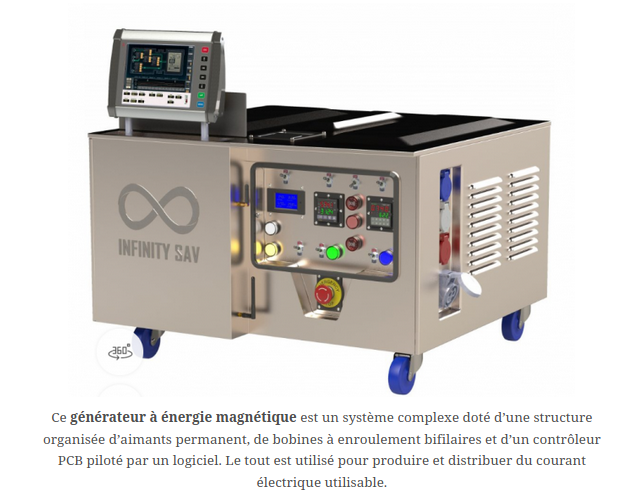
\includegraphics[width=.7\linewidth]{generateur_energie_libre.png}
    \caption{Un exemple très élaboré de canular... ou d'arnaque pour ceux qui l'achètent.}
    \label{generateur_energie_libre}
\end{figure}

\newpage

\section{Exercices}
\begin{exercise}
    Une tige de longueur l et un cadre rectangulaire de largueur l sont lâchés ensemble et tombent dans un champ magnétique uniforme. Y'a-t-il une différence dans leur mouvement ? On suppose que le cadre n'est jamais entièrement dans le champ.
    \begin{figure}[h!]
        \centering
        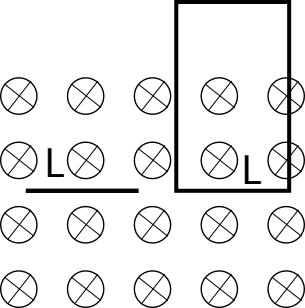
\includegraphics[width=.4\linewidth]{exe_induction_1.png}
        \label{loi_faraday_1}
    \end{figure}
\end{exercise}

\begin{exercise}
    Le plan d'un cadre de dimension 12cmx7cm est initialement perpendiculaire à un champ magnétique uniforme de \(0,2[T]\). Déterminez la variation de flux à travers le cadre lorsqu'il tourne de \(120^{\circ}\) autour d'un axe perpendiculaire aux lignes de champ.
    Commence par faire un schéma \enquote{vu de haut} présentant le vecteur surface te les lignes de champ dans la situation initiale puis la situation finale.
\end{exercise}

\begin{exercise}
    Le plan d'une spire circulaire de rayon 6cm fait un angle de \(30^{\circ}\) avec un champ magnétique uniforme de \(0,25[T]\).
    \begin{enumerate}[a)]
        \item Quel est le flux à travers la spire ?
        \item Si on inverse le sens du champ, quelle est la variation de flux ?
    \end{enumerate}
\end{exercise}

\begin{exercise}
    Un solénoïde comportant 10 spires/cm est parcouru par un courant de 4[A]. À l'intérieur du solénoïde se trouve une bobine de 5 spires, de section \(A=8cm^2\) et dont l'axe fait un angle de \(37^{\circ}\) avec celui du premier solénoïde. Déterminez la valeur de la tension induite si le courant augmente de 25 \% en 0,1 s.
\end{exercise}

\begin{exercise}
    Une tige métallique de longueur l=5cm se déplace à vitesse constante v sur des rails de résistance négligeable formant un circuit fermé avec une résistance R=0,2[Ohms] (rail de Laplace). Un champ magnétique sortant constant et uniforme B=0,25[T] est normal au plan des rails. Un courant induit de I=2[A] circule dans le sens horloger.
    \begin{enumerate}[a)]
        \item Que vaut la vitesse ?
        \item Quelle force faut-il exercer sur la tige pour la déplacer à vitesse constante ?
    \end{enumerate}
\end{exercise}

\begin{exercise}
    Un cadre carré de 3 cm de côté tourne avec une fréquence de 5[Hz] dans un champ magnétique uniforme de 0,5[T] perpendiculaire à la surface du cadre. Si une résistance électrique de 1,5[Ohms] est branché sur le cadre, quelle quantité de chaleur ce dispositif émet-il à chaque seconde ?
\end{exercise}

\begin{exercise}
    On place une bobine carrée mesurant 5cm de côté et comportant 100 spires perpendiculairement à un champ magnétique uniforme de 0,6[T]. On l'en éloigne ensuite rapidement et d'un mouvement régulier (elle reste toujours perpendiculaire au champ) jusqu'à une zone où l'intensité de B est brusquement nulle. Ce déplacement dure 0,1[s].

    \begin{enumerate}[a)]
        \item Que vaut la tension induite ?
        \item Si la tension induite s'oppose à une résistance de 100 Ohm, que vaut l'intensité du courant ?
        \item Quelle quantité d'énergie est dissipée sous forme de chaleur durant ce déplacement ?
    \end{enumerate}
\end{exercise}
